\chapter{Quantum Networking With an Elementary Operating System}
\label{chp:qnodeos}

\begin{abstract}
An \acrfull{os} for quantum network nodes should provide more than just networking functionalities.
Ultimately, it should enable quantum networking applications to be written in high-level,
platform independent software, and should be able to manage the resources of the underlying
device when deployed in a multi-node and multi-user quantum network. This chapter briefly
discusses our implementation of \acrshort{qnodeos}, an \acrshort{os} for quantum network nodes,
which includes a quantum network stack for entanglement generation, as well as resource
management and scheduling features that allow the concurrent execution of multiple applications.
We also validate our implementation on state-of-the-art quantum network hardware based on
\acrlong{nv} centers in diamond, and discuss general design considerations for any such quantum
network \acrshort{os}. Our work sets a baseline for running applications on quantum networks
of the future, and serves as a hands-on study to understand and define computer-science
challenges in building quantum network \acrshortpl{os}.
\end{abstract}

\noindent
\note{To be precise, this chapter is extracted from sections 5 (Implementation), 6 (Evaluation), 7
(Related Work) and 8 (Discussion) from the \acrshort{qnodeos} paper. There aren't any major
additions.}

\blfootnote{
    This chapter is based on the preprint \fullcite{delledonne_2023_qnodeos_noprint}. \note{Add
    proper link to arXiv when submitted}
}

\newpage

\lettrine{T}{he} preliminary experiments conducted in \cref{chp:netstack} showcased elementary
quantum networking functionalities through a platform-independent control system --- mainly, the
quantum networking stack embedded in \acrshort{qnodeos}. Nevertheless, entanglement generation is
just one of the blocks constituting fully-fledged quantum communications applications, which also
include local quantum processing and classical communication and processing, as shown in
\cref{fig:app-struct}. With \acrshort{qnodeos}, we aim to take the state of the art of quantum
networking experiments one step further, and demonstrate the execution of complete applications,
some of which comprise quantum and classical processing and communication. We also include one case
study that serves as a proof-of-concept demonstration of the usefulness of a multitasking-ready
\acrshort{os}, to be expanded on when investigating multi-user quantum networks more in depth. In
this chapter we report on and discuss the results of these experiments. Prior to that, we also give
a brief overview of the implementation of \acrshort{qnodeos} and the underlying \acrshort{qdevice}.
Refer to \cref{app:qnodeos} for additional details on the implementation of the components of
\acrshort{qnodeos} and their interfaces, and to \cref{app:qdevice} for the specification of the
interface to the \acrshort{qdevice}.

\section{Implementation}
\label{sec:qnodeos:implementation}

\Cref{fig:node-deployment} outlines software and hardware implementation of \acrshort{qnodeos} and
the whole node system. \acrshort{qnodeos} is implemented in C++ on top of FreeRTOS, a tiny operating
system for microcontrollers~\cite{freertos}. The stack runs on a dedicated MicroZed~\cite{microzed}
--- an off-the-shelf platform based on the Zynq-7000 SoC, which hosts two ARM Cortex-A9 processing
cores, of which only one is used, clocked at \qty{667}{\MHz}. \acrshort{qnodeos} connects to peer
\acrshort{qnodeos} systems via \acrshort{tcp} over a Gigabit Ethernet interface. For the
\acrshort{qdevice}, we replicated the setup used for \cref{chp:netstack}, which mainly consists of:
%
\begin{inlinelist}
    \item an ADwin-Pro II~\cite{adwin} acting as the main orchestrator of the setup;
    \item a series of subordinate devices responsible for qubit control, including laser pulse
          generators and optical readout circuits;
    \item the quantum physical device, based on \acrshort{nv} centers, counting one single
          (communication) qubit for each node.
\end{inlinelist}
The \acrshort{qdevice} is where the time-critical qubit control lies. \acrshort{qnodeos} interfaces
with the \acrshort{qdevice}'s ADwin-Pro II through a \qty{12.5}{\MHz} \acrshort{spi} interface, used
to exchange 4-byte control messages at a rate of \qty{50}{kHz}. Finally, the host layer is a Python
runtime executing on a general-purpose 4-core desktop machine running Linux. The host machine
connects to \acrshort{qnodeos} via \acrshort{tcp} over the same Gigabit Ethernet interface that
\acrshort{qnodeos} uses to connect to its peers (average ping \acrshort{rtt} of \qty{0.1}{\ms}), and
sends application registration requests and quantum code blocks over this interface (\num{10} to
\num{1000} bytes, depending on the length of the block).

We implemented \acrshort{qnodeos} on top of FreeRTOS to avoid re-implementing standard \acrshort{os}
primitives like threads and network communication. FreeRTOS provides basic \acrshort{os}
abstractions like tasks, inter-task message passing, and the \acrshort{tcpip} stack. The FreeRTOS
kernel --- like any other standard \acrshort{os} --- cannot however directly manage the quantum
resources (qubits, entanglement requests and entangled pairs), and hence its task scheduler cannot
take decisions based on such resources. \acrshort{qnodeos} adds these capabilities and takes care of
the scheduling of quantum code blocks based on the status of the quantum resources.

\begin{figure}[t]
    \centering
    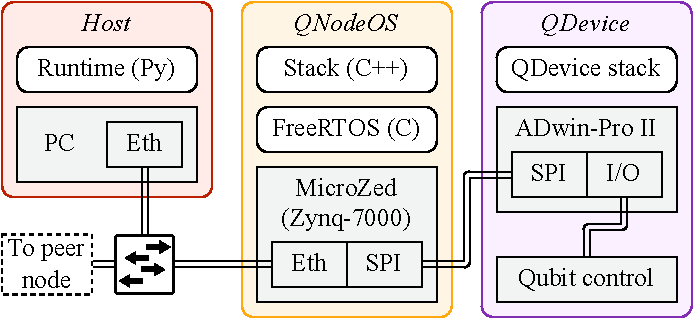
\includegraphics[width=0.6\linewidth]{figures/node-deployment.pdf}
    \caption{
        Node deployment overview. Our quantum network node consists of a desktop machine for the
        host runtime, a Zynq-7000 SoC for \acrshort{qnodeos}, and a series of digital and analog
        controllers for the \acrshort{qdevice}.
    }
    \label{fig:node-deployment}
\end{figure}

\section{Evaluation}
\label{sec:qnodeos:evaluation}

We verify the functioning of \acrshort{qnodeos} by means of four case studies, aimed at validating
\begin{inlinelist}
    \item single-node execution, including qubit initialization, gates, and measurements,
    \item entanglement generation,
    \item delegated quantum computation, and
    \item multitasking.
\end{inlinelist}

\subsection{Local Qubit State Tomography}

Our first case study is a simple local application where a certain qubit state is prepared and then
immediately measured. This translates to one or more single-qubit gates and one qubit measurement.
The application is run several times to assess the quality of the prepared state, and various qubit
states are analyzed. This local qubit state tomography is the simplest application
\acrshort{qnodeos} can run --- there is a single user process running, and the network process is
not even activated, given that entanglement is never requested.

\paragraph{Results}

This application prepares the six cardinal states $\ket{+X}$, $\ket{+Y}$, $\ket{+Z}$, $\ket{-X}$,
$\ket{-Y}$, and $\ket{-Z}$, in sequence. Each state is measured in all six cardinal bases. This
application is run \num{1000} times for each combination of target state and readout basis. The
measured state fidelity, reported in \cref{fig:local-tomo}, is in line with what the quantum
hardware is capable of delivering, showing that basic interactions among the components of
\acrshort{qnodeos} and with the \acrshort{qdevice} work.

\begin{figure}[t]
    \centering
    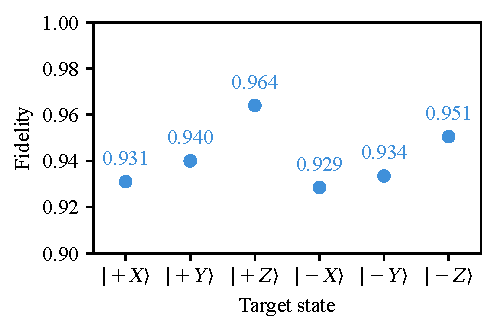
\includegraphics[width=0.6\linewidth]{figures/local-tomography.pdf}
    \caption{
        Average fidelity of the prepared cardinal states $\ket{+X}$, $\ket{+Y}$, $\ket{+Z}$,
        $\ket{-X}$, $\ket{-Y}$, and $\ket{-Z}$ in the local qubit state tomography application.
    }
    \label{fig:local-tomo}
\end{figure}

\subsection{Entanglement Generation}

The second test case is an application that generates an entangled pair between the two nodes and
measures the generated state right away. This is a distributed application, where both nodes are
active --- they engage in entanglement generation, and they both measure their end of the entangled
pair. As the user can specify the requested fidelity of the entangled pairs, this application is run
for various target fidelities. This time, all \acrshort{qnodeos} components are at work. Since
entanglement is requested, the quantum network stack is triggered, and thus the network process
becomes active, competing for resources with the user process. The \acrshort{qmmu} is also invoked
by the network process to transfer ownership of the entangled qubit to the user process (the
inter-process communication primitive of \acrshort{qnodeos}).

\paragraph{Results}

Entanglement generation is run for a range or target fidelities \numlist{0.50; 0.55; 0.60; 0.65;
0.70; 0.75; 0.80}, and entangled pairs are read out in various bases to measure their correlators
$\braket{\mathrm{XX}}$, $\braket{\mathrm{YY}}$ and $\braket{\mathrm{ZZ}}$ (and their $\pm$
variations, for a total of $12$ correlators). The application is run \num{125} times for each
combination of target fidelity and correlator, for a total of \num{10500} entangled pairs. The
results for measured fidelity versus requested fidelity are shown in \cref{fig:ent-gen}. The
measured fidelities are --- within measurement uncertainty --- always matching or exceeding the
requested minimum ones (the dashed gray line in \cref{fig:ent-gen} is the $y=x$ diagonal). It is to
be noted that measurement outcomes are post-processed to eliminate tomography errors and events in
which the physical devices were in the incorrect charge state.
\note{Retake this experiment, fidelities have gotten worse on setup. Also report on fidelities
without correction.}

\begin{figure}[t]
    \centering
    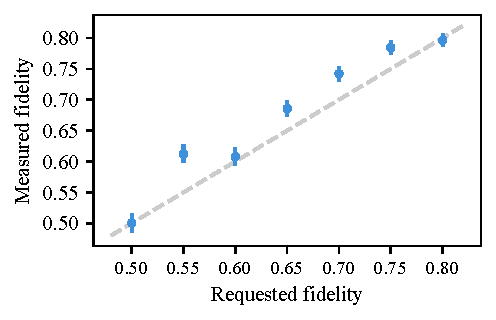
\includegraphics[width=0.6\linewidth]{figures/ent-gen.pdf}
    \caption{
        Measured fidelity of the entangled states generated and read out via \acrshort{qnodeos}.
        Measurements are corrected to eliminate tomography errors and events in which the physical
        devices were in the incorrect charge state. Error bars represent 1 s.d. The dashed gray line
        is the $y=x$ diagonal.
    }
    \label{fig:ent-gen}
\end{figure}

\subsection{Delegated Computation}

With this case study we aim to showcase a more complex quantum network application, schematically
depicted in \cref{fig:del-comp}. Here, one node acts as the client, and the other as the server. The
client's goal is to delegate a certain quantum computation on some data qubit to the server, while
keeping the server agnostic to the computation. To perform the desired computation, described by a
parameter $\alpha$, the two nodes follow these steps:
%
\begin{inlinelist}
    \item the two node establish an entangled state,
    \item the client ``encodes'' its qubit by means of a series of local gates, described by a
          parameter $\theta$,
    \item the client measures its end of the entangled pair and stores the classical outcome
          $m_\text{c}$
    \item the client communicates the delegated computation parameter, which is a function of
          $\alpha$, $\theta$ and $m_\text{c}$,
    \item the server performs the computation,
    \item the server measures its end of the entangled pair and sends the classical outcome
          $m_\text{s}$ back to the client.
\end{inlinelist}
In this scheme, the client application consists of a single quantum code block and an additional
classical code block that communicates the computation parameter to the server. More interestingly,
the server application comprises two quantum code blocks --- the first is the establishment of the
entangled pair, and the second is the delegated computation --- interleaved by a classical code
block that receives the computation parameter from the client. This is the first example of an
interactive application, where the execution (on the server) spans more than one quantum code block,
and thus the quantum state generated in one block has to persist and remain valid for the other
block too.

\begin{figure}[t]
    \centering
    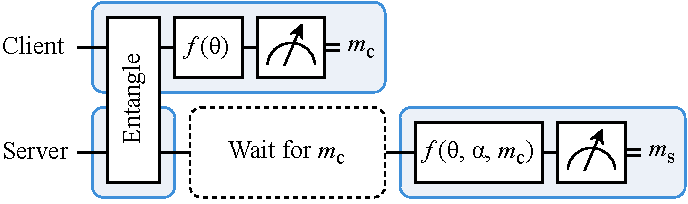
\includegraphics[width=0.6\linewidth]{figures/del-comp.pdf}
    \caption{
        Schematic of delegated computation application. The client wishes to have the server perform
        a quantum computation on a certain data qubit. To do so, the two nodes establish
        entanglement, then the client processes and measures its end of the entangled pair, sends
        the computation parameter to the server, which finally executes the delegated computation.
        Blue boxes represent quantum code blocks. The client's application is composed of a single
        block, while the server's consists of one block for entanglement and one block for the
        quantum computation, interleaved by a classical code block (the reception of the computation
        parameter).
    }
    \label{fig:del-comp}
\end{figure}

\paragraph{Results}

\note{Refine when data is available.}
The delegated computation is run for various values of $\alpha$ ($\pi$, $\pi/2$) and $\theta$
($\pi$, $\pi/2$, $\pi/4$). The application is run \num{500} times for each combination of $\alpha$
and $\theta$. We report the measured fidelity of the qubit state after the delegated computation for
each of the computation values. We also report a breakdown of the average application latency, to
give an indication of where time is spent during execution. [...] The abstractions provided by
\acrshort{qnodeos} allow for the execution of more complex quantum network applications. Distributed
applications may result in idle time on some nodes, which \acrshort{qnodeos} can allocate to other
pending applications.

\subsection{Multitasking}

One of the core features of modern \acrshortpl{os} is the ability to run several applications
concurrently, a key aspect in multi-user networks and nodes. \acrshort{qnodeos} is designed with
multitasking capabilities --- not only can it multiplex a user process and the network process, but
it also allows for multiple user processes to run at the same time. This means that multiple users
can submit their applications simultaneously, and \acrshort{qnodeos} will service all pending user
processes based on resource availability, in order to increase the utilization of the
\acrshort{qdevice} and to limit idle time and average application latency. One drawback of
multitasking on a quantum network node is the trade-off between concurrency and fidelity:
applications that have active data in the quantum memory, and that are waiting to be scheduled while
other applications are in progress, may experience lower-quality qubit states, given that such
quality degrades due to the passing of time and to noise induces by operations on other qubits.

We aim to demonstrate the multitasking capabilities of \acrshort{qnodeos} by having multiple users
run independent applications concurrently. In our case study, a pool of users runs the delegated
computation application, while the rest of the users runs the local qubit state tomography
application. We evaluate multitasking on the client node, while the server just runs its part of the
delegated computation application. The idle time resulting from running the delegated computation
application on the client is a perfect candidate for scheduling other pending applications. We
evaluate the multitasking performance of \acrshort{qnodeos} under various system load conditions,
which essentially depend on the number of users utilizing \acrshort{qnodeos} at the same time. We
note that, even though a higher degree of concurrency should in principle results in better device
utilization, this is limited by the scarce physical resources available on the underlying
\acrshort{qdevice}.

\paragraph{Results}

\note{Refine when data is available.}
We measure device utilization and average application latency on the client, for various
configurations of users and applications: $N$ users, with $N \in \{2, 3, 5, 10\}$, half of which
running the local tomography application, and the remaining half running the delegated computation
application. To measure the performance benefit of multitasking, we also run the same set of
applications with multitasking disabled --- on \acrshort{qnodeos}, this means that a user process
can only be scheduled if no other user processes are either running or waiting for entanglement
generation. We report device utilization and average application latency, for the various usage
patters, resulting from a continuous execution of each usage pattern over \qty{\approx 30}{min}.
[...] The scheduler of \acrshort{qnodeos}, in combination with the \acrshort{qmmu}, can dynamically
re-prioritize outstanding processes based on resource availability. \acrshort{qnodeos} can thus
support multi-user quantum network nodes, and can take advantage of network idle times to improve
device utilization and average application latency. Impact of multitasking on fidelity not visible
with a single qubit.

\section{Related Work}
\label{sec:qnodeos:relwork}

Relative to quantum networking, a substantial amount of software and systems work happens in the
field of quantum computing. For example, operating systems for quantum computers (without networking
functionality) are under active development in research and industry~\cite{kong_2021_origin,
deltaflow_os}. Furthermore, extensive work exists on developing quantum computing
architectures~\cite{fu_2017_microarch, murali_2019_fullstack, bourassa_2021_blueprint}. In this
work, we have addressed new problems that arise specifically from the inclusion of quantum
networking which has not been considered at all in the aforementioned \acrshortpl{os} and
publications.

Nevertheless, systems research in quantum networking has been growing as a field as well. In
particular, over the past several years there have been multiple proposals for quantum network
protocol stacks~\cite{van_meter_2013_repeaters, pirker_2019_quantum, dahlberg_2019_egp,
illiano_2022_quantum} and quantum network architectures~\cite{matsuo_2019_bootstrapping,
aguado_2020_enabling, li_2022_connectionless, diadamo_2022_packet, pouryousef_2022_overlay,
gu_2023_fendi, mandil_2023_packet}. One of the proposed network stacks has even been demonstrated
experimentally on a state-of-the-art two-node network in a lab~\cite{pompili_2022_experimental} ---
as detailed in \cref{chp:netstack} --- while the rest has only been validated in simulation.
However, these works heavily focus on the network protocol aspects and whilst some of them
acknowledge that the stacks will exist as a component in a bigger system, they do not tackle any of
the related issues, such as resource management or task scheduling.

Quantum network applications themselves have also been demonstrated on small networks in
laboratories~\cite{barz_2012_demonstration}. However, such demonstrations have always been \emph{ad
hoc}, and scripted through low-level experimental controls as their purpose was to demonstrate
hardware technology milestones rather than develop general systems for multiple users.

\section{Discussion}

\noindent
\note{Copy over from \acrshort{qnodeos} paper after experiments have been performed}

\printbibliography[heading=subbibintoc,title={References},notcategory=noprint]
